% Generazione delle variabili che andranno a sostituire quelle del template `HomePage.tex`
\newcommand{\documento}{\PdP}
\newcommand{\nomedocumentofisico}{PianoDiProgetto\_v1\_0\_0.pdf}
\newcommand{\redazione}{\TG \\ & \LC}
\newcommand{\verifica}{\NC \\ & \SG \\ & \MM}
\newcommand{\approvazione}{\CV}
\newcommand{\versione}{1.0.0}
\newcommand{\uso}{Esterno}
\newcommand{\destinateTo}{\TV, \\ & \RC, \\ & \II}
\newcommand{\datacreazione}{28 novembre 2018}
\newcommand{\datamodifica}{28 novembre 2018}
\newcommand{\stato}{Approvato}

\def\TABELLE{false}	% abilita - disabilita l'indice delle tabelle
\def\FIGURE{false} 	% abilita - disabilita l'indice delle figure

% Layout del documento 
\documentclass[a4paper,11pt]{article}

\usepackage{ifthen}
\usepackage[english,italian]{babel}
\usepackage[utf8]{inputenc}
\usepackage[T1]{fontenc}
\usepackage{float}
\usepackage{chapterbib}
\usepackage{graphicx}
\usepackage[a4paper,top=2.5cm,bottom=2.5cm,left=2.5cm,right=2.5cm]{geometry}

\PassOptionsToPackage{hyphens}{url}\usepackage[hyperfootnotes=false]{hyperref}
\hypersetup{%
	colorlinks=true,
	citecolor=black,
	linkcolor=black,
	urlcolor=blue
}

\usepackage{enumitem}
\usepackage{eurosym}
\usepackage{booktabs}
\usepackage{fancyhdr}
\usepackage{totpages}
\usepackage{tabularx, array}
\usepackage{dcolumn}
\usepackage{epstopdf}
\usepackage{booktabs}
\usepackage{fancyhdr}
\usepackage{longtable}
\usepackage{calc}
\usepackage{datatool}
\usepackage[bottom]{footmisc}
\usepackage{listings}
\usepackage{textcomp}
\usepackage{titlesec}
\usepackage{rotating}
\usepackage{multirow}
\usepackage{placeins}
\usepackage{color}
\usepackage{makecell}
\usepackage{lscape}
 
\usepackage[table,usenames,dvipsnames]{xcolor}
% Definizione di nuovi colori da poter usare per le tabelle
\definecolor{lightgray}{gray}{0.92}
\definecolor{lightblue}{rgb}{0.93,0.95,1.0}
\definecolor{headgray}{gray}{0.88}

% Ridefinizione dell'env tabularx. Il vecchio è utilizzabile con l'env oldtabularx
\let\oldtabularx\tabularx
\let\endoldtabularx\endtabularx
\renewenvironment{tabularx}{\rowcolors{2}{white}{lightgray}\oldtabularx}{\endoldtabularx}

% Per tabularx con padding, parametro tra [], eg [1.3]
\newenvironment{paddedtablex}[1][1]{%
	\renewcommand*{\arraystretch}{#1}%
	\renewcommand\theadfont{\bfseries}%
	\tabularx%
}{%
	\endtabularx
}

% Ridefinizione dell'env tabular. Il vecchio è utilizzabile con l'env oldtabular
\let\oldtabular\tabular
\let\endoldtabular\endtabular
\renewenvironment{tabular}{\rowcolors{2}{lightgray}{white}\oldtabular}{\endoldtabular}

% Per tabular con padding, parametro tra [], eg [1.3]
\newenvironment{paddedtable}[1][1]{%
	\renewcommand*{\arraystretch}{#1}%
	\renewcommand\theadfont{\bfseries}%
	\tabular%
}{%
	\endtabular
}

% ***TABELLA ANALISI RISCHI PDP***

\newenvironment{risktable}[1][1]{%
	\centering%
	\renewcommand*{\arraystretch}{1.4}%
	\renewcommand\theadfont{\bfseries}%
	\oldtabularx%
}{%
	\endoldtabularx
}

% ***TABELLA SUDDIVISIONE DEL LAVORO PDP***

\newenvironment{detailtable}[1][1]{%
	\centering%
	\renewcommand*{\arraystretch}{1.4}%
	\renewcommand\theadfont{\bfseries}%
	\oldtabularx%
}{%
	\endoldtabularx
}

% ***TABELLA ORGANIGRAMMA***

\newenvironment{orgtable}[1][1]{%
	\centering%
	\renewcommand*{\arraystretch}{1.4}%
	\renewcommand\theadfont{\bfseries}%
	\oldtabularx%
}{%
	\endoldtabularx
}


% DA SPOSTARE SU COMANDI
% ***DOUBLE LINE***

\def\mydoublerule#1#2#3{%%
	\hrule width#1 height#2 \vskip#2
	\hrule width#1 height#3 
}

% ***NUOVO TIPO DI CELLA CENTRATA***

\newcolumntype{Y}{>{\centering\arraybackslash}X}

% ***STILE PAGINA***
\pagestyle{fancy}

% ***INTESTAZIONE***
\rhead{\Large{\progetto} \\ \footnotesize{\documento}}
\lhead{
\includegraphics[keepaspectratio = true, width = 25px]{../template/icons/a6(1).png}}

% ***PIÈ DI PAGINA***
\lfoot{\textit{\gruppo} \\
\footnotesize{\email}}

\rfoot{\thepage} % per le prime pagine: mostra solo il numero romano
\cfoot{}
\renewcommand{\footrulewidth}{0.4pt}   % Linea sopra il piè di pagina
\renewcommand{\headrulewidth}{0.4pt}  % Linea sotto l'intestazione

% ***INSERIMENTO DI NUOVE SOTTOSEZIONI
\setcounter{secnumdepth}{7} %mostra nel documento fino al livello 8 (1.2.3.4.5.6.7.8)
\setcounter{tocdepth}{7}    % mostra nell'indice fino al livello 8 (1.2.3.4.5.6.7.8)


\makeatletter
\newcounter{subsubparagraph}[subparagraph]
\renewcommand\thesubsubparagraph{%
	\thesubparagraph.\@arabic\c@subsubparagraph}
\newcommand\subsubparagraph{%
	\@startsection{subsubparagraph}    % counter
	{6}                              % level
	{\parindent}                     % indent
	{3.25ex \@plus 1ex \@minus .2ex} % beforeskip
	{0.75em}                           % afterskip
	{\normalfont\normalsize\bfseries}}
\newcommand\l@subsubparagraph{\@dottedtocline{6}{10em}{5.5em}} %gestione dell'indice
\newcommand{\subsubparagraphmark}[1]{}
\makeatother

\makeatletter
\newcounter{subsubsubparagraph}[subsubparagraph]
\renewcommand\thesubsubsubparagraph{%
	\thesubsubparagraph.\@arabic\c@subsubsubparagraph}
\newcommand\subsubsubparagraph{%
	\@startsection{subsubsubparagraph}    % counter
	{7}                              % level
	{\parindent}                     % indent
	{3.25ex \@plus 1ex \@minus .2ex} % beforeskip
	{0.75em}                           % afterskip
	{\normalfont\normalsize\bfseries}}
\newcommand\l@subsubsubparagraph{\@dottedtocline{7}{10em}{6.5em}} %gestione dell'indice
\newcommand{\subsubsubparagraphmark}[1]{}
\makeatother


\addtocounter{vZ}{1}
\newcommand{\modifiche}
{
	% \addToDiary{Inserimento qualità di processo}{\Ver}{\NC}{03-01-2018}
	% \addToDiary{Inserimento qualità di prodotto}{\Ver}{\NC}{30-12-2018}
	% \addToDiary{Inserimento standard ISO 90003}{\Ver}{\NC}{27-12-2018}
	% \addToDiary{Inserimento standard ISO 9126}{\Ver}{\NC}{26-12-2018}
	% \addToDiary{Inserimento standard ISO 15504}{\Ver}{\NC}{23-12-2018}
	
	\addToDiary{Aggiunto appendice \S{C} (mitigazione variazioni)}{\Ver}{\MM}{14-02-2019}

	% 1.Y.Z
	\setcounter{vX}{1}%
	\setcounter{vY}{0}%
	\setcounter{vZ}{0}%

	\addToDiary{Approvazione per il rilascio}{\Res}{\NC}{13-01-2019}

	% 0.2.Z
	\decrvX
	\setcounter{vY}{2}%
	\setcounter{vZ}{0}%

	\addToDiary{Verifica finale}{\Ver}{\MM}{12-01-2019}

    % 0.1.Z
    \decrvY%
	\setcounter{vZ}{2}%

	\addToDiary{Aggiunto appendice ``Valutazioni per il miglioramento''}{\Ver}{\MM}{11-01-2019}
	\addToDiary{Inserito ``Resoconto delle attività di verifica''}{\Ver}{\NC}{08-01-2019}
	\addToDiary{Verifica documento}{\Ver}{\CV}{10-12-2018}

    % 0.0.Z
	\setcounter{vZ}{5}%
	\decrvY%

	\addToDiary{Aggiunto appendice ``Standard di qualità''}{\Ver}{\NC}{03-12-2018}
	\addToDiary{Inserito ``Qualità di processo''}{\Ver}{\NC}{02-12-2018}
	\addToDiary{Inserito ``Qualità di prodotto''}{\Ver}{\TG}{01-12-2018}
	\addToDiary{Aggiunta Introduzione}{\Ver}{\NC}{29-11-2018}
    \addToDiary{Creazione template}{\Red}{\TG}{27-11-2018}
}



% Comandi generali
% Generali
\newcommand{\progetto}{Butterfly}
\newcommand{\gruppo}{AlphaSix}
\newcommand{\email}{alpha.six.unipd@gmail.com}

% Documenti
\newcommand{\AdR}{Analisi dei Requisiti}
\newcommand{\NdP}{Norme di Progetto}
\newcommand{\PdP}{Piano di Progetto}
\newcommand{\SdF}{Studio di Fattibilità}
\newcommand{\PdQ}{Piano di Qualifica}
\newcommand{\VI}{Verbale Interno}
\newcommand{\VE}{Verbale Esterno}
\newcommand{\ST}{Specifica Tecnica}
\newcommand{\DDP}{Definizione di Prodotto}
\newcommand{\MU}{Manuale Utente}
\newcommand{\Gl}{Glossario}
\newcommand{\LdP}{Lettera di Presentazione}
\newcommand{\AdRv}{AnalisiDeiRequisiti v2.0.0}
\newcommand{\NdPv}{NormeDiProgetto v2.0.0}
\newcommand{\PdPv}{PianoDiProgetto v2.0.0}
\newcommand{\PdQv}{PianoDiQualifica v2.0.0}
\newcommand{\SdFv}{StudioDiFattibilità v1.0.0}
\newcommand{\DdPv}{DefinizioneDiprodotto v1.0.0}
\newcommand{\Glv}{Glossario v2.0.0}

% Componenti del gruppo
\newcommand{\LC}{Laura Cameran}
\newcommand{\TG}{Timoty Granziero}
\newcommand{\CV}{Ciprian Voinea}
\newcommand{\SG}{Samuele Gardin}
\newcommand{\NC}{Nicola Carlesso}
\newcommand{\MM}{Matteo Marchiori}

% Ruoli
\newcommand{\RdP}{Responsabile di Progetto}
\newcommand{\Res}{Responsabile}
\newcommand{\Red}{Redattore}
\newcommand{\Amm}{Amministratore}
\newcommand{\Ver}{Verificatore}
\newcommand{\Prog}{Progettista}
\newcommand{\Progr}{Programmatore}
\newcommand{\Ana}{Analista}
\newcommand{\RdPs}{Responsabili di Progetto}
\newcommand{\Ress}{Responsabile}
\newcommand{\Amms}{Amministratori}
\newcommand{\Vers}{Verificatori}
\newcommand{\Progs}{Progettisti}
\newcommand{\Progrs}{Programmatori}
\newcommand{\Anas}{Analisti}

% Professori e proponente
\newcommand{\TV}{Prof. Tullio Vardanega}
\newcommand{\RC}{Prof. Riccardo Cardin}
\newcommand{\LuC}{Luca Cappelletti}
\newcommand{\DZ}{Davide Zanetti}
\newcommand{\II}{Imola Informatica}
\newcommand{\proponente}{Imola Informatica}

% Comando per una nuova riga nella tabella del diario delle modifiche
\newcommand{\specialcell}[2][c]{%
	\begin{tabular}[#1]{@{}c@{}}#2\end{tabular}}

\renewcommand*\sectionmark[1]{\markboth{#1}{}}
\renewcommand*\subsectionmark[1]{\markright{#1}}

% Pediodi di lavoro 
\newcommand{\AR}{Analisi dei Requisiti}
\newcommand{\AD}{Analisi dei Requisiti in Dettaglio}
\newcommand{\PA}{Progettazione Architetturale}
\newcommand{\PD}{Progettazione di Dettaglio}
\newcommand{\CO}{Codifica}
\newcommand{\VV}{Validazione}

% Revisioni
\newcommand{\RR}{Revisione dei Requisiti}
\newcommand{\RP}{Revisione di Progettazione}
\newcommand{\RQ}{Revisione di Qualifica}
\newcommand{\RA}{Revisione di Accettazione}

\newcommand{\myincludegraphics}[2][]{%
	\setbox0=\hbox{\phantom{X}}%
	\vtop{
		\hbox{\phantom{X}}
		\vskip-\ht0
		\hbox{\includegraphics[#1]{#2}}}}

% Ridefinizione linea per le note a piè di pagina
\renewcommand{\footnoterule}{%
  \kern -3pt
  \hrule width \textwidth height 0.4pt
  \kern 2pt
}

\colorlet{punct}{red!60!black}
\definecolor{background}{HTML}{EEEEEE}
\definecolor{delim}{RGB}{20,105,176}
\colorlet{numb}{magenta!60!black}
\lstdefinelanguage{json}{
 	basicstyle=\small\ttfamily,
 	numbers=left,
 	numberstyle=\scriptsize,
 	stepnumber=1,
 	numbersep=8pt,
 	showstringspaces=false,
 	breaklines=true,
 	frame=lines,
 	backgroundcolor=\color{background},
 	literate=
 	*{0}{{{\color{numb}0}}}{1}
 	{1}{{{\color{numb}1}}}{1}
 	{2}{{{\color{numb}2}}}{1}
 	{3}{{{\color{numb}3}}}{1}
 	{4}{{{\color{numb}4}}}{1}
 	{5}{{{\color{numb}5}}}{1}
 	{6}{{{\color{numb}6}}}{1}
 	{7}{{{\color{numb}7}}}{1}
 	{8}{{{\color{numb}8}}}{1}
 	{9}{{{\color{numb}9}}}{1}
 	{:}{{{\color{punct}{:}}}}{1}
 	{,}{{{\color{punct}{,}}}}{1}
 	{\{}{{{\color{delim}{\{}}}}{1}
 	{\}}{{{\color{delim}{\}}}}}{1}
 	{[}{{{\color{delim}{[}}}}{1}
 	{]}{{{\color{delim}{]}}}}{1},
}
\lstset{language=json}
\lstset{literate=%
    {Ö}{{\"O}}1
 	{Ä}{{\"A}}1
 	{Ü}{{\"U}}1
 	{é}{{\"s}}1
 	{è}{{\"e}}1
 	{à}{{\"a}}1
	{ö}{{\"o}}1
}


\definecolor{listinggray}{gray}{0.9}
\definecolor{lbcolor}{rgb}{0.9,0.9,0.9}

\lstset{
  backgroundcolor=\color{lbcolor},
  tabsize=4,
  language=Python,
  captionpos=b,
  frame=single,
  numbers=left,
  numberstyle=\tiny,
  numbersep=5pt,
  breaklines=true,
  showstringspaces=false,
  basicstyle=\footnotesize,
  % identifierstyle=\color{magenta},
  keywordstyle=\bfseries\color[rgb]{0,0,1},
  commentstyle=\color[rgb]{0,0.6,0},
  stringstyle=\color{red}
}

% \definecolor{mygreen}{rgb}{0,0.6,0}
% \definecolor{mygray}{rgb}{0.5,0.5,0.5}
% \definecolor{mymauve}{rgb}{0.58,0,0.82}

% \lstset{ 
%   backgroundcolor=\color{white},   % choose the background color; you must add \usepackage{color} or \usepackage{xcolor}; should come as last argument
%   basicstyle=\footnotesize,        % the size of the fonts that are used for the code
%   breakatwhitespace=false,         % sets if automatic breaks should only happen at whitespace
%   breaklines=true,                 % sets automatic line breaking
%   captionpos=b,                    % sets the caption-position to bottom
%   commentstyle=\color{mygreen},    % comment style
%   deletekeywords={...},            % if you want to delete keywords from the given language
%   escapeinside={\%*}{*)},          % if you want to add LaTeX within your code
%   extendedchars=true,              % lets you use non-ASCII characters; for 8-bits encodings only, does not work with UTF-8
%   firstnumber=1000,                % start line enumeration with line 1000
%   frame=single,	                   % adds a frame around the code
%   keepspaces=true,                 % keeps spaces in text, useful for keeping indentation of code (possibly needs columns=flexible)
%   keywordstyle=\color{blue},       % keyword style
%   language=Octave,                 % the language of the code
%   morekeywords={*,...},            % if you want to add more keywords to the set
%   numbers=left,                    % where to put the line-numbers; possible values are (none, left, right)
%   numbersep=5pt,                   % how far the line-numbers are from the code
%   numberstyle=\tiny\color{mygray}, % the style that is used for the line-numbers
%   rulecolor=\color{black},         % if not set, the frame-color may be changed on line-breaks within not-black text (e.g. comments (green here))
%   showspaces=false,                % show spaces everywhere adding particular underscores; it overrides 'showstringspaces'
%   showstringspaces=false,          % underline spaces within strings only
%   showtabs=false,                  % show tabs within strings adding particular underscores
%   stepnumber=2,                    % the step between two line-numbers. If it's 1, each line will be numbered
%   stringstyle=\color{mymauve},     % string literal style
%   tabsize=2,	                   % sets default tabsize to 2 spaces
%   title=\lstname                   % show the filename of files included with \lstinputlisting; also try caption instead of title
% }

\newcommand{\impl}{\textcolor{Green}{Implementato}}
\newcommand{\implno}{\textcolor{Red}{Non Implementato}}

% G di glossario a pedice, con e senza spazio
\newcommand{\GAlt}{\ped{\tiny{G}}}
\newcommand{\G}{\ped{\tiny{G }}}

% e.g. \gloss{progetto}
\newcommand{\gloss}[1]{%
    {\small \textsc{#1}}\GAlt%
}

% D di documento a pedice, con e senza spazio
% \newcommand{\DAlt}{\ped{\tiny{D}}}
\newcommand{\D}{\ped{\tiny{D}}}

% e.g. \Doc{Norme di Progetto}
\newcommand{\Doc}[1]{\textit{#1}\D}

% Comandi per applicare \Doc con un comando unico
\newcommand{\PdQd}{\Doc{\PdQv}}
\newcommand{\PdPd}{\Doc{\PdPv}}
\newcommand{\NdPd}{\Doc{\NdPv}}
\newcommand{\AdRd}{\Doc{\AdRv}}
\newcommand{\SdFd}{\Doc{\SdFv}}
\newcommand{\Gld}{\Doc{\Gld}}

% Le sottosezioni paragraph, subparagraph ecc.. vengono visualizzate come section
\titleformat{\paragraph}{\normalfont\normalsize\bfseries}{\theparagraph}{1em}{}
\titlespacing*{\paragraph}{0pt}{3.25ex plus 1ex minus .2ex}{1.5ex plus .2ex}

\titleformat{\subparagraph}{\normalfont\normalsize\bfseries}{\thesubparagraph}{1em}{}
\titlespacing*{\subparagraph}{0pt}{3.25ex plus 1ex minus .2ex}{1.5ex plus .2ex}

\titleformat{\subsubparagraph}{\normalfont\normalsize\bfseries}{\thesubsubparagraph}{1em}{}
\titlespacing*{\subsubparagraph}{0pt}{3.25ex plus 1ex minus .2ex}{1.5ex plus .2ex}

\titleformat{\subsubsubparagraph}{\normalfont\normalsize\bfseries}{\thesubsubsubparagraph}{1em}{}
\titlespacing*{\subsubsubparagraph}{0pt}{3.25ex plus 1ex minus .2ex}{1.5ex plus .2ex}


% Indentazione paragrafi rimossa. Per metterla manualmente, precedere il paragrafo con il comando /indent
\newlength\tindent
\setlength{\tindent}{\parindent}
\setlength{\parindent}{0pt}
\renewcommand{\indent}{\hspace*{\tindent}}


% Generazione automatica dei numeri per le versioni
\newcounter{vX} % valore per X in X.Y.Z
\newcounter{vY} % valore per Y in X.Y.Z
\newcounter{vZ} % valore per Z in X.Y.Z
\newcommand{\decrvX}{\addtocounter{vX}{-1}} % Comando per il decremento automatico del counter vZ
\newcommand{\decrvY}{\addtocounter{vY}{-1}} % Comando per decrementare vY
\newcommand{\decrvZ}{\addtocounter{vZ}{-1}} % Comando per decrementare vZ
\newcommand{\addToDiary}[4]{\thevX.\thevY.\thevZ & #1 & #2 & #3 & #4\decrvZ\\} % Comando per generare una riga di diario delle modifiche (\addToDiary{desc}{ruolo}{nominativo}{data})

% Colore righe grigie
\newcommand{\tablegray}{gray!20}

% Stile liste
% \renewcommand\labelitemi{$\circ$} % Bullet, primo livello
% \renewcommand\labelitemii{$\diamond$} % Bullet, primo livello
% \renewcommand\labelitemii{\normalfont\bfseries \textendash} % --, secondo livello
% \renewcommand\labelitemiii{\textasteriskcentered} % *, terzo livello
% \renewcommand\labelitemiv{\textperiodcentered} % ., quarto livello
% \setlist[itemize,2]{label=$\circ$}
% \setlist[itemize,2]{label=$\diamond$}

% Placeholder sui diari
\newcommand{\pl}{Placeholder}

%Comandi per le versioni delle tecnologie
\newcommand{\python}{Python 3.6.7}
\newcommand{\gitlab}{GitLab 11.7}
\newcommand{\redmine}{Redmine 4.0.1}
\newcommand{\kafka}{Apache Kafka 2.12}
\newcommand{\docker}{Docker 18.09}
\newcommand{\telegram}{Telegram (Bot API 4.0)}
\newcommand{\slack}{Slack}
\newcommand{\jenkins}{Jenkins 2.146}




\begin{document}
	
    % Inclusione template HomePage
    \begin{center}

%\includegraphics[width=1em]{../../../Template/icone/LogoGruppo.png}
\begin{large} \textbf{\progetto} \end{large}
%\includegraphics[width=1em]{../../../Template/icone/LogoGruppo.png}
\vspace{0.2em}

\hrule
\vspace{7em}


\includegraphics[keepaspectratio = true, width=5cm]{../template/icons/sotto.png}

%Prima pagina senza intestazione né piè di pagina	
\thispagestyle{empty}

%spazio tra il nome e il logo
\vspace{1.5em}

%Copertina
\begin{center} 
  \begin{Huge}
  {\fontsize{15mm}{20mm}\selectfont \gruppoLink} 
  \end{Huge}
\end{center}

%Le informazioni del documento sono ancorate a fine pagina
\vfill

\begin{Huge} \documento \end{Huge}

\begin{center}
% \textbf{Informazioni sul documento} \\ \vspace{2em}
% \small
\begin{tabular}{r|l}
	\multicolumn{2}{c}{\textbf{Informazioni sul documento} } \\ \hline
	\textbf{Nome Documento} & \nomedocumentofisico \\
	% \textbf{Versione} & \versione \\
	\textbf{Data di Creazione} & \datacreazione \\
	\textbf{Data ultima modifica} & \datamodifica \\
	\textbf{Stato} & \stato \\
	\textbf{Redazione} & \redazione \\
	\textbf{Verifica} & \verifica \\
	\textbf{Approvazione} & \approvazione \\
	\textbf{Uso} & \uso \\
	\textbf{Distribuzione} & \gruppo \\
	\textbf{Destinato a} & \destinateTo \\
	\textbf{Email di riferimento} & \email
\end{tabular}
\end{center}

\normalsize

% Sommario
\textbf{Descrizione} \\
Questo documento fornisce la definizioni di alcuni dei termini apparsi in altri documenti allegati redatti 
da \gruppo\ durante lo svolgimento del progetto Butterfly, con
lo scopo di evitare ogni forma di ambiguit\`a.
 

%\vfill
\end{center}

\clearpage

    % Registro delle modifiche e indice
    % si usa la numerazione romana per gli indici e la tabella delle modifiche
    \pagenumbering{Roman}
    \addtocounter{vZ}{1}
\newcommand{\modifiche}
{
	% \addToDiary{Inserimento qualità di processo}{\Ver}{\NC}{03-01-2018}
	% \addToDiary{Inserimento qualità di prodotto}{\Ver}{\NC}{30-12-2018}
	% \addToDiary{Inserimento standard ISO 90003}{\Ver}{\NC}{27-12-2018}
	% \addToDiary{Inserimento standard ISO 9126}{\Ver}{\NC}{26-12-2018}
	% \addToDiary{Inserimento standard ISO 15504}{\Ver}{\NC}{23-12-2018}
	
	\addToDiary{Aggiunto appendice \S{C} (mitigazione variazioni)}{\Ver}{\MM}{14-02-2019}

	% 1.Y.Z
	\setcounter{vX}{1}%
	\setcounter{vY}{0}%
	\setcounter{vZ}{0}%

	\addToDiary{Approvazione per il rilascio}{\Res}{\NC}{13-01-2019}

	% 0.2.Z
	\decrvX
	\setcounter{vY}{2}%
	\setcounter{vZ}{0}%

	\addToDiary{Verifica finale}{\Ver}{\MM}{12-01-2019}

    % 0.1.Z
    \decrvY%
	\setcounter{vZ}{2}%

	\addToDiary{Aggiunto appendice ``Valutazioni per il miglioramento''}{\Ver}{\MM}{11-01-2019}
	\addToDiary{Inserito ``Resoconto delle attività di verifica''}{\Ver}{\NC}{08-01-2019}
	\addToDiary{Verifica documento}{\Ver}{\CV}{10-12-2018}

    % 0.0.Z
	\setcounter{vZ}{5}%
	\decrvY%

	\addToDiary{Aggiunto appendice ``Standard di qualità''}{\Ver}{\NC}{03-12-2018}
	\addToDiary{Inserito ``Qualità di processo''}{\Ver}{\NC}{02-12-2018}
	\addToDiary{Inserito ``Qualità di prodotto''}{\Ver}{\TG}{01-12-2018}
	\addToDiary{Aggiunta Introduzione}{\Ver}{\NC}{29-11-2018}
    \addToDiary{Creazione template}{\Red}{\TG}{27-11-2018}
}

    % Inserisce il link all'indice
% \addcontentsline{toc}{section}{Indice}

\tableofcontents
\clearpage 

% Se è stata impostata a true la variabile per la lista delle tabelle, la mostra
\ifthenelse{\equal{\TABELLE}{true}} 
{\listoftables}{}

% Se è stata impostata a true la variabile per la lista delle figure, la mostra
\ifthenelse{\equal{\FIGURE}{true}}
{\listoffigures}{}

% Da qui comincia la numerazione normale
\pagenumbering{arabic}
\setcounter{page}{1}

% Imposta il formato di visualizzazione
\rfoot{\thepage~di~\pageref{TotPages}}
    % \newpage
    % \listoffigures
    % \newpage
    % \listoftables
    % \newpage

    % Sezioni documento
    \newpage
\section{Introduzione} \label{Introduzione}
	
	\subsection{Scopo del documento}
	Questo documento ha l'intento di specificare la pianificazione e l'approccio che AlphaSix adotterà per portare a termine il progetto Butterfly.
	All'interno vengono illustrate le strategie, le suddivisioni dei compiti, l'utilizzo delle risorse, la gestione dei rischi e le attività secondo le quali il gruppo ha intenzione di lavorare.
	
	\subsection{Scopo del prodotto}	
	Il prodotto che AlphaSix si incarica di realizzare è composto da ... tool per prendere i messaggi , tool per analizzarli e mandarli verso gestore interno o direttamente alle perosne interessate tramite canale di informazione che è stato scelto ...
	
	\subsection{Glossario}
		\subsubsection{Riferimenti Normativi}
			\begin{itemize}
				\item Capitolato d'appalto C1 (aggiungere link)
				\item Vincoli di organigramma (aggiungere link a sito di tullio)
				\item Norme di progetto interne di AlphaSsix 
				\item The twelve factor app, https://12factor.net/, consigliato fortemente dall'azienda
			\end{itemize}
		
		\subsubsection{Riferimenti Informativi}
			\begin{itemize}
				\item Software engineering di sommerville
				\item slide di tullio
			\end{itemize}
		
	\subsection{Scadenze}
	Il gruppo ha deciso di rispettare le scadenze indicate dal professor Vardanega e riportate di seguito:
	\begin{itemize}
		\item Revisione dei Requisiti: 2012-12-21;
		\item Revisione di Progetto: 2013-02-03;
		\item Revisione di Qualifica: 2013-03-06;
		\item Revisione di Accettazione: 2013-03-16.
	\end{itemize}
	
	\subsection{Ciclo di vita}
	Il gruppo ha deciso di adottare il modello incrementale come ciclo di vita da adottare per i processi in quanto si adatta particolarmente per questo progetto.
	Ogni ripetizione del ciclo identifica un "ciclo di incremento": questo verrà ripetuto fino a quando il prodotto non arriverà a soddisfare interamente i requisiti richiesti dal cliente.
	Questa decisione è stata presa in quanto:
	\begin{itemize}
		\item le richieste presentate nel capitolato sono facilmente scomponibili in sottoproblemi categorizzabili in base alla loro importanza e di conseguenza possono essere soddisfatti partendo da quelli più critici a quelli meno critici anche parallelamente
		\item il passaggio da un incremento ad un altro consolida il processo appena concluso riducendo il rischio di fallimento e facilitando la verifica parziale del prodotto
		\item la ripartizione in cicli permette un controllo più efficente delle risorse pianificandone l'uso
	\end{itemize}
	Addottando questa modalità il gruppo può rilasciare al committente un prototipo (funzionale) che soddisfa requisiti più importanti fra quelli presentati nel capitolato.
	
	Inizialmente quindi si potranno spendere le risorse nella realizzazione di una base (baseline) che possa presentare il core del prodotto finale.
	
	A tale base(line) saranno successivamente integrate le funzionalità secondarie richieste dal cliente nel capitolato e secondo la pianificazione e le risorse disponibili potranno essere aggiunte altre funzionalità opzionali e desidarabili che possono sorgere nello svuiluppo del prodotto o nel durante delle analisi dei requisiti (da rivedere tutto il paragrafo)
	 
    \newpage
\section{Analisi dei rischi} \label{AnalisiDeiRischi}
	
	Per sviluppare il progetto in maniera efficiente ed efficace viene effettuata un'analisi preliminare dei rischi che possono creare problemi nel processo di sviluppo.
	E' quindi fondamentale avere un sistema che ne permetta la gestione in modo da poter agire immediatamente e con un piano ben definito in caso dovessero presentarsi.
	I seguenti punti rappresentano come il gruppo ha deciso di trattare i rishi:
	
	\begin{itemize}
		\item Identificazione: individuare i potenziali rischi che possono presentarsi
		\item Analisi e valutazione: determinarne la probabilità di occorrenza e comprenderne la criticità
		\item Pianificazione: si definiscono strategie che possono evitare i rischi precendentemente trovati
		\item Controllo: si monitorano e revisionano i rischi finche il progetto procede 
		\item Revisione: in caso dovessero presentarsi rischi (anche imprevisti), dopo averli risolti si rivede la strategia utilizzata e si rivede e migliora in caso qualcosa non ha funzionato come si deve o ci fosse la possibilità
	\end{itemize}
	
	\subsection{Classi di gravità}
	
	Per l'identificazione dei rischi viene utilizzato come strumento di misura la tabella del qualitative risk assessment, in modo da dare a ciascun rischio un valore ben preciso per e catalogarli dal meno al più rischioso.
	
	\begin{center}
		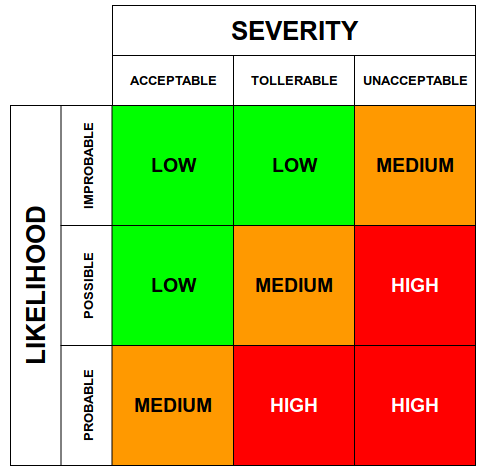
\includegraphics[scale=0.5]{img/tabella.png}
	\end{center}


	I rischi che possono esserci all'interno del progetto rientrano in queste categorie
	
	Di seguito verranno elencati i rischi analizzati dal gruppo nel seguente modo:\\
	
	\begin{table}[H]
		\begin{risktable}{\columnwidth}{m{1.5cm}m{4.1cm}m{4.1cm}m{4.1cm}}
			\thead{ID} & 
			\thead{Probabilità} & 
			\thead{Gravità} & 
			\thead{Classe} \\
			\hline
			\multicolumn{4}{X}{
				\thead{Nome}
			}\\
			\hline
			\multicolumn{4}{X}{
				\thead{Descrizione}
			}\\
			\hline
			\multicolumn{4}{X}{
				\thead{Mitigazione}
			}\\
		\end{risktable}
		\caption{Fac simile tabella rischi}
	\end{table}
	
	Lista rischi possibili: 
	
	\begin{table}[H]
		\begin{risktable}{\columnwidth}{m{1.5cm}m{4.1cm}m{4.1cm}m{4.1cm}}
			ID & 
			Probabilità & 
			Gravità &
			Classe\\
			\hline
			\multicolumn{4}{X}{
				Impreparazione del team a livello tecnico
			}\\
			\hline
			\multicolumn{4}{X}{
				Non tutti i componenti del gruppo hanno le conoscenze di ambienti di sviluppo, linguaggi di programmazione e strumenti richiesti dall'azienda allo stesso livello
			}\\
			\hline
			\multicolumn{4}{X}{
				Le ore di studio peronale si usano per portare il gruppo ad un livello di conoscenza comune
			}\\
		\end{risktable}
	\end{table}

	\mydoublerule{\linewidth}{0pt}{2pt}

	\begin{table}[H]
		\begin{risktable}{\columnwidth}{m{1.5cm}m{4.1cm}m{4.1cm}m{4.1cm}}
			ID & 
			Probabilità & 
			Gravità &
			Classe\\
			\hline
			\multicolumn{4}{X}{
				Impreparazione del team a livello gestionale
			}\\
			\hline
			\multicolumn{4}{X}{
				Non avendo affrontato progetti del genere prima d'ora, i componenti del gruppo non conoscono bene i ruoli che devono intraprendere e i compiti che devono svolgere
			}\\
			\hline
			\multicolumn{4}{X}{
				Durante le ore di studio personale non rendicontate ciascun componente si impegna a studiare la gerarchia dei ruoli fornita nel materiale del professore in modo da essere preparati quando si cambia di ruolo.
				Inoltre, coloro che ricopriranno i ruoli di responsabile e amministratore saranno attenti a controllare che gli altri rispettino i compiti del ruolo a loro assegnato.
			}\\
		\end{risktable}
	\end{table}
	
		\mydoublerule{\linewidth}{0pt}{2pt}
		
\begin{table}[H]
		
		\begin{risktable}{\columnwidth}{m{1.5cm}m{4.1cm}m{4.1cm}m{4.1cm}}
			ID & 
			Probabilità & 
			Gravità &
			Classe\\
			\hline
			\multicolumn{4}{X}{
				Non arrivare giusti ad una scadenza
			}\\
			\hline
			\multicolumn{4}{X}{
				Descrizione
			}\\
			\hline
			\multicolumn{4}{X}{
				Mitigazione
			}\\
		\end{risktable}
	\end{table}
	
	\mydoublerule{\linewidth}{0pt}{2pt}
\begin{table}[H]
		
		\begin{risktable}{\columnwidth}{m{1.5cm}m{4.1cm}m{4.1cm}m{4.1cm}}
			ID & 
			Probabilità & 
			Gravità & 
			Classe\\
			\hline
			\multicolumn{4}{X}{
				Errore di approvazione dei documenti
			}\\
			\hline
			\multicolumn{4}{X}{Durante la fase di approvazione dei documenti p possibile che ci siano degli errori da parte di chi ha il ruolo di responsabile nell'approvazione dei documenti, questo può portare alla consegna di documentazione errata o fatta male che può causare disguidi col cliente (oltre che brutta figura) e necessità di rivedere i documenti, quindi spreco di risorse.}\\
			\hline
			\multicolumn{4}{X}{Colui che al momento svolge il ruolo di respoonsavie deve assicurarsi che i documenti che approva siano effettivamente validi e in caso ci fossero errori da parte sua il verificatore deve saper trovare ed in caso correggere tali errori.}\\
		\end{risktable}
	\end{table}
	
	\mydoublerule{\linewidth}{0pt}{2pt}
	
	\begin{table}[H]
		
		\begin{risktable}{\columnwidth}{m{1.5cm}m{4.1cm}m{4.1cm}m{4.1cm}}
			ID & 
			Probabilità & 
			Gravità & 
			Classe\\
			\hline
			\multicolumn{4}{X}{
				Cattiva gestione dell'archivio di documentazione di progetto
			}\\
			\hline
			\multicolumn{4}{X}{
				DESCRIZIONE
			}\\
			\hline
			\multicolumn{4}{X}{
				
				Organizzare una repo comune in cui ciascun componente può caricare il proprio lavoro
				
				chi fa il ruolo di amministratore deve leggersi per bene cosa deve fare e come svolgere il proprio compito, cosa manca da fare su ciascun documento ---> monitoraggio del lavoro di stesura dei documenti da parte degli altri componenti del gruppo
			}\\
		\end{risktable}
		
	\end{table}

	\mydoublerule{\linewidth}{0pt}{2pt}
	
	\begin{table}[H]
		
		\begin{risktable}{\columnwidth}{m{1.5cm}m{4.1cm}m{4.1cm}m{4.1cm}}
			ID & 
			Probabilità & 
			Gravità & 
			Classe\\
			\hline
			\multicolumn{4}{X}{
				NOME
			}\\
			\hline
			\multicolumn{4}{X}{
				Non ci si conosce tra membri e differenze nello stile di lavoro
			}\\
			\hline
			\multicolumn{4}{X}{
				il gruppo all'inizio si è preso cura di conoscersi e parlare e capire le preferenze di ciascun membro e la sua preparazione
			}\\
		\end{risktable}
		
	\end{table}
	
	\mydoublerule{\linewidth}{0pt}{2pt}
\begin{table}[H]
		
		\begin{risktable}{\columnwidth}{m{1.5cm}m{4.1cm}m{4.1cm}m{4.1cm}}
			ID & 
			Probabilità & 
			Gravità & 
			Classe\\
			\hline
			\multicolumn{4}{X}{
				Impegni personali e universitari da gestire in parallelo al progetto
			}\\
			\hline
			\multicolumn{4}{X}{
				DESCRIZIONE
			}\\
			\hline
			\multicolumn{4}{X}{
				sarà compito del responsabile coordinare gli incontri e la spartizione del lavoro in modo tale da assicurare la buona collaborazione di ciascun membro in modo equo
			}\\
		
		\end{risktable}
	\end{table}
	
	\mydoublerule{\linewidth}{0pt}{2pt}
	
	\begin{table}[H]
		
		\begin{risktable}{\columnwidth}{m{1.5cm}m{4.1cm}m{4.1cm}m{4.1cm}}
			ID & 
			Probabilità & 
			Gravità & 
			Classe\\
			\hline
			\multicolumn{4}{X}{
				Problematiche hardware
			}\\
			\hline
			\multicolumn{4}{X}{
				esplosione computer
			}\\
			\hline
			\multicolumn{4}{X}{
				MITIGAZIONE
			}\\
		\end{risktable}
	\end{table}
	
	\mydoublerule{\linewidth}{0pt}{2pt}
	
	\begin{table}[H]
		
		\begin{risktable}{\columnwidth}{m{1.5cm}m{4.1cm}m{4.1cm}m{4.1cm}}
			ID & 
			Probabilità & 
			Gravità & 
			Classe\\
			\hline
			\multicolumn{4}{X}{
				Aggiunta o modifica di requisiti in corso di sviluppo
			}\\
			\hline
			\multicolumn{4}{X}{
				DESCRIZIONE
			}\\
			\hline
			\multicolumn{4}{X}{
				siccome il progetto è facilmente suddivisibile in più sottoproblemi con basso livello di accopiamento, l'aggiunta o modifica di requisiti non dovrebbe andare a impattare (modularità) come vengono gestiti e sviluppati gli altri requisiti, si aggiungono costi che andranno a modificare il preventivo e quindi tempo perso, vengono rispartite le risorse e i assegnate ai nuovi ruoli che verranno ricoperti dai membri del team
			}\\
		\end{risktable}
		
	\end{table}
	
	\mydoublerule{\linewidth}{0pt}{2pt}
	
	\begin{table}[H]
		
		\begin{risktable}{\columnwidth}{m{1.5cm}m{4.1cm}m{4.1cm}m{4.1cm}}
			ID & 
			Probabilità & 
			Gravità & 
			Classe\\
			\hline
			\multicolumn{4}{X}{
				Problematiche software
			}\\
			\hline
			\multicolumn{4}{X}{
				errore di vario tipo, vedere sweefty
			}\\
			\hline
			\multicolumn{4}{X}{
				MITIGAZIONE
			}\\
		\end{risktable}
		
	\end{table}

	\mydoublerule{\linewidth}{0pt}{2pt}
	
	\begin{table}[H]
		
		\begin{risktable}{\columnwidth}{m{1.5cm}m{4.1cm}m{4.1cm}m{4.1cm}}
			ID & 
			Probabilità & 
			Gravità & 
			Classe\\
			\hline
			\multicolumn{4}{X}{
				Interpretazione errata delle requisiti presenti
			}\\
			\hline
			\multicolumn{4}{X}{
				errore di vario tipo, vedere sweefty
			}\\
			\hline
			\multicolumn{4}{X}{
				{nel capitolato}(migliore analisi iniziale e riflessione più approfondita sulle richieste dell'azienda)
			}\\
		\end{risktable}
		
	\end{table}
	
	\mydoublerule{\linewidth}{0pt}{2pt}

	\begin{table}[H]
		
		\begin{risktable}{\columnwidth}{m{1.5cm}m{4.1cm}m{4.1cm}m{4.1cm}}
			ID & 
			Probabilità & 
			Gravità & 
			Classe\\
			\hline
			\multicolumn{4}{X}{
				Mancanza di comunicazione con l'azienda 
			}\\
			\hline
			\multicolumn{4}{X}{
				errore di vario tipo, vedere sweefty
			}\\
			\hline
			\multicolumn{4}{X}{
				 (richieste di incontro via skype e invio di report ogni tot tempo, richiesta di incontri con azienda, molta comunicazione tra cliente e fornitore)
			}\\
		\end{risktable}
		
	\end{table} 	

	\mydoublerule{\linewidth}{0pt}{2pt}
	
	\begin{table}[H]
		
		\begin{risktable}{\columnwidth}{m{1.5cm}m{4.1cm}m{4.1cm}m{4.1cm}}
			ID & 
			Probabilità & 
			Gravità & 
			Classe\\
			\hline
			\multicolumn{4}{X}{
				Spreco di risorse
			}\\
			\hline
			\multicolumn{4}{X}{
				errore di vario tipo, vedere sweefty
			}\\
			\hline
			\multicolumn{4}{X}{
					 (continuo monitoraggio tramite diagrammi gantt) parlare di zero laxity e zero latency
			}\\
		\end{risktable}
		
	\end{table} 
	
	[fare oltre ai diagrammi a colonne, anche i diagrammi a torta]
	
	\subsection{Livello tecnologico}
	\subsubsection{Tecnologie adottate}
	\subsubsection{Rotture Hardware}
	
	\subsection{Livello del personale}
	\subsubsection{Problemi dei componenti del gruppo}
	\subsubsection{Problemi tra componenti del gruppo}
	\subsubsection{Inesperienza del gruppo}
	
	\subsection{Livello organizzativo e di valutazione dei costi}
	\subsection{Livello dei requisiti}

    \newpage
\section{Pianificazione} \label{Pianificazione}
	La fase di Pianificazione consiste nella suddivisione del lavoro. Questsa deve fare in modo che ogni componente del gruppo abbia la possibilità di ricoprire almeno una volta tutti i ruoli del progetto. È stato deciso dal gruppo di utilizzare lo standard ISO/IEC 12207:1995, questo prevede l'utilizzo della seguente struttura:
	\begin{itemize}
			\item Analisi
			\item Progettazione
			\item Realizzazione
			\item Manutenzione
		\end{itemize}
	Per rendere più chiara l'idea utilizzeremo vari diagrammi di Gantt dove sarà chiaro chi ha svolto qualsiasi attività.	
		\subsection{Analisi vista dall'alto / generale}
		
		Questa attività ha inizio il 15-11-2018 e termina il 21-01-2019. In questa fase i ruoli attivi saranno: 
		\begin{itemize}
			\item Project Manager
			\item Amministratore
			\item Analista
			\item Verificatore
		\end{itemize}
		In questo periodo le attività svolte saranno:
		\begin{itemize}
			\item \textbf{Norme di progetto:} questa attività spetta all'Amministratore. Egli dovrà stipulare una serie di norme che dovrannno essere rispettate dai componenti del gruppo per tutta la durata del progetto. Le quali sono interne al gruppo e non legate al capitolato scelto. Questa attività deve essere svolta a priori così da garantire uno standard per la stesura dei doumenti e per quanto riguarda le tecnologie usate.
			\item \textbf{Studio di fattibilità:} questa attività valuta rischi, costi e benefici dei vari capitolati proposti. Viene svolta dagli Analisti e in base ad un accurato studio emergono pro e contro di ogni capitolato. Questi dati sono vari e spesso incerti. Una volta analizzati, portano alla scelta definitiva del capitolato da implementare. L'attività risulta bloccante per l'inizio della stesura dell'Analisi dei requisiti.
			\item \textbf{Analisi dei requisiti:} questa attività richiede un grande approfondimento dei requisiti. questi devono essere soddisfacibili, necessari e sufficenti. Questa responsabilità spetta agli Analisti. 
			\item \textbf{Piano di progetto:} questa attività viene svolta dal Responsabile che avendo bene in mente le scadenze analizza le attività necessarie, l'Amministratore invece studierà i rischi che il gruppo potrà dover affrontare durante lo svolgimento del progetto. L'obbiettivo è quello di organizzare attività con efficenza per produrre risultati efficaci.
			\item \textbf{Piano di qualifica:} questa attività è svolta dagli Amministratori, dove vengono studiate le strategie di verifca e validazione adottate.
			\item \textbf{Glossario:} questa attività viene svlota dai redattori. Consiste nell'inserimento di termini che protrebbero risultare ambigui, così aiuta a garantire una terminologia consistente.
			\item \textbf{Lettera di presentazione:} questa attività consiste nella stesura del documento dove il gruppo AlphaSix si presenta come Fornitore del prodotto richiesto.
		\end{itemize}
		
			\subsubsection{Diagramma di gantt}
			\subsubsection{WBS (Work Breakdown Structure)}
			\subsubsection{Ripartizione delle ore}
				vedere don't panic, hanno messo una tabella con ore ripartite
				Secondo me questa sezione comprende la parte di studio personale messa da sweefty
				
		\subsection{Analisi in dettaglio}
			\subsubsection{Diagramma di gantt}
			\subsubsection{WBS (Work Breakdown Structure)}
			\subsubsection{Ripartizione delle ore}

		\subsection{Progettazione architetturale}
			\subsubsection{Diagramma di gantt}
			\subsubsection{WBS (Work Breakdown Structure)}
			\subsubsection{Ripartizione delle ore}
			
		\subsection{progettazione di dettaglio e codifica}
			\subsubsection{Diagramma di gantt}
			\subsubsection{WBS (Work Breakdown Structure)}
			\subsubsection{Ripartizione delle ore}
			
		\subsection{Verifica e validazione}
			\subsubsection{Diagramma di gantt}
			\subsubsection{WBS (Work Breakdown Structure)}
			\subsubsection{Ripartizione delle ore}
			
		

    % Secondo me da togliere, cade sotto pianificazione (CV)
    % \newpage
\section{Calendario attivita} \label{CalendarioAttivita}

	Lorem ipsum dolor sit amet, consectetur adipiscing elit, sed do eiusmod tempor incididunt ut labore et dolore magna aliqua. Ut enim ad minim veniam, quis nostrud exercitation ullamco laboris nisi ut aliquip ex ea commodo consequat. Duis aute irure dolor in reprehenderit in voluptate velit esse cillum dolore eu fugiat nulla pariatur. Excepteur sint occaecat cupidatat non proident, sunt in culpa qui officia deserunt mollit anim id est laborum.
	
	\subsection{Consegne}
		\subsubsection{Tabella date}

	Da fare con gantt, vedere anche altri gruppi, sweefty a meno che non sia una cosa fatta nel paragrafo precedente

	Contiene scritto impegno del gruppo a consegare a tot date e per tot scadenze
    \newpage
\section{Suddivisione del lavoro} \label{SuddivisioneDelLavoro}

	Lorem ipsum dolor sit amet, consectetur adipiscing elit, sed do eiusmod tempor incididunt ut labore et dolore magna aliqua. Ut enim ad minim veniam, quis nostrud exercitation ullamco laboris nisi ut aliquip ex ea commodo consequat. Duis aute irure dolor in reprehenderit in voluptate velit esse cillum dolore eu fugiat nulla pariatur. Excepteur sint occaecat cupidatat non proident, sunt in culpa qui officia deserunt mollit anim id est laborum.

	\subsection{Dettaglio Fasi}
		\subsubsection{Analisi}
		\subsubsection{Analisi Dettaglio}
		\subsubsection{Progettazione Architetturale}
		\subsubsection{Progettazione di Dettaglio e Codifica}
		\subsubsection{Verifica e Validazione}

	\subsection{Totali}
		\subsubsection{Ore totali con investimento}	
    \newpage
\section{Prospetto economico} \label{ProspettoEconomico}

	Lorem ipsum dolor sit amet, consectetur adipiscing elit, sed do eiusmod tempor incididunt ut labore et dolore magna aliqua. Ut enim ad minim veniam, quis nostrud exercitation ullamco laboris nisi ut aliquip ex ea commodo consequat. Duis aute irure dolor in reprehenderit in voluptate velit esse cillum dolore eu fugiat nulla pariatur. Excepteur sint occaecat cupidatat non proident, sunt in culpa qui officia deserunt mollit anim id est laborum.
	
	Preso da don't panic

	\subsection{Analisi}
	\subsection{Analisi Dettaglio}
	\subsection{Progettazione Architetturale}
	\subsection{Progettazione di Dettaglio e Codifica}
	\subsection{Verifica e Validazione}
	\subsection{Totale}
		\subsubsection{Ore totali con investimento}
		\subsubsection{Ore rendicontate}
		\subsubsection{Conclusioni}
    \newpage
\section{Consuntivo (e preventivo?) a finire}

	Lorem ipsum dolor sit amet, consectetur adipiscing elit, sed do eiusmod tempor incididunt ut labore et dolore magna aliqua. Ut enim ad minim veniam, quis nostrud exercitation ullamco laboris nisi ut aliquip ex ea commodo consequat. Duis aute irure dolor in reprehenderit in voluptate velit esse cillum dolore eu fugiat nulla pariatur. Excepteur sint occaecat cupidatat non proident, sunt in culpa qui officia deserunt mollit anim id est laborum.

	Vedere sweefty
	
	\subsection{Analisi dei Requisiti}
		\subsubsection{Consuntivo}
		\subsubsection{Conclusioni}
	
	
    \newpage
\section{Controllo e rendicontazione} \label{ControlloERendicontazione}

	Lorem ipsum dolor sit amet, consectetur adipiscing elit, sed do eiusmod tempor incididunt ut labore et dolore magna aliqua. Ut enim ad minim veniam, quis nostrud exercitation ullamco laboris nisi ut aliquip ex ea commodo consequat. Duis aute irure dolor in reprehenderit in voluptate velit esse cillum dolore eu fugiat nulla pariatur. Excepteur sint occaecat cupidatat non proident, sunt in culpa qui officia deserunt mollit anim id est laborum.

	\subsection{title}
		\subsubsection{title}
		
		
	Vedere come altri gruppi hanno aggiunto tabelle con firme di tutti i componenti

    % \appendix
    \newpage
\section{Organigramma}
	
	\subsection{Redazione}
	\begin{table}[H]
		\centering
		\begin{oldtabular}{|c|c|c|}
			\hline
			\thead{Nome} &\thead{Data} &\thead{Firma} \\
			\hline	
			\CV & 2018-01-06 & A  \\
			\hline
		\end{oldtabular}
		\caption{Redazione}
	\end{table}

	\subsection{Approvazione}
	\begin{table}[H]
		\centering
		\begin{oldtabular}{|c|c|c|}
			\hline
			\thead{Nome} &\thead{Data} &\thead{Firma} \\
			\hline			
			\CV & 2018-01-08 & A  \\
			\hline
			Tullio Vardanega &  &  \\
			\hline
			Riccardo Cardin &  &  \\
			\hline
		\end{oldtabular}
		\caption{Approvazione}
	\end{table}

	\subsection{Accettazione componenti}
	\begin{table}[H]
		\centering
		\begin{oldtabular}{|c|c|c|}
			\hline
			\thead{Nome} &\thead{Data} &\thead{Firma} \\
			\hline
			\CV & 2018-01-10 & A  \\
			\hline
			\LC & 2018-01-10 & A \\
			\hline
			\SG & 2018-01-10 & A \\
			\hline
			\MM & 2018-01-10 & A \\
			\hline
			\NC & 2018-01-10 & A \\
			\hline
			\TG  & 2018-01-10 & A \\
			\hline
		\end{oldtabular}
		\caption{Accettazione componenti}
	\end{table}

	\begin{table}[H]
		\centering
		\begin{paddedtable}[1.3]{ccc}
			\thead{Nome} & \thead{Data} & \thead{Firma} \\
			\toprule
			\CV & 2018-01-10 & A  \\
			\LC & 2018-01-10 & A \\
			\SG & 2018-01-10 & A \\
			\MM & 2018-01-10 & A \\
			\NC & 2018-01-10 & A \\
			\TG  & 2018-01-10 & A \\
			\bottomrule
		\end{paddedtable}
		\caption{Accettazione componenti}
	\end{table}

	Aaggungere colonna ruoli ricoperti da ciascuna persona
	\subsection{Componenti}	
	\begin{table}[H]
		\centering
		\begin{oldtabular}{|c|c|c|}
			\hline
			\thead{Nome} & \thead{Matricola} &\thead{Indirizzo} \\
			\hline			
			\CV & 2018-01-10 & A  \\
			\hline
			\LC & 2018-01-10 & A \\
			\hline
			\SG & 2018-01-10 & A \\
			\hline
			\MM & 2018-01-10 & A \\
			\hline
			\NC & 2018-01-10 & A \\
			\hline
			\TG  & 2018-01-10 & A \\
			\hline
		\end{oldtabular}
		\caption{Componenti}
	\end{table}

	\subsection{Definizione dei ruoli}
		Nel corso dello sviluppo del progetto i membri del gruppo si impegneranno a ricorpire diversi ruoli che rappresentano figure aziendali specializzate indispensabili per la riuscita del progetto e per la qualità del prodotto finale.
		Ciascun componente del gruppo dovrà ricoprire almeno una volta ogni ruolo in modo tale che non ci siano sovrapposizioni di compiti e che chi ricopre il ruolo di verificatore non vada a controllare il proprio lavoro ma sempre quello altrui.
		Ci possono essere più persone che ricoprono lo stesso ruolo in uno stesso momento.
		Questi ruoli sono:	
		\begin{itemize}
			\item Responsabile
			\item Amministratore
			\item Analista
			\item Progettista
			\item Programmatore
			\item Verificatore
		\end{itemize}
		
		\begin{table}[H]
			\centering
			\begin{oldtabular}{|c|c|c|}
				\hline
				\thead{Ruolo} &\thead{Costo} \\
				\hline	
				Responsabile & \EUR{30} \\
				\hline
				Amministratore & 20 \\
				\hline
				Analista & 25 \\
				\hline
				Progettista & 22 \\
				\hline
				Programmatore & 15 \\
				\hline
				Verificatore & 15 \\
				\hline
			\end{oldtabular}
			\caption{Costo \euro/h per ciascun ruolo}
		\end{table}

\end{document}